\begin{pastexam}[label={px:ntu-113-dsa-05}]{臺大資工所 113 學年度 第 5 題}
（複選；每個選項單獨計分）

(10 points) A Binary Search Tree (abbreviated as BST) is a tree structure comprised of nodes that
maintain a specific order among their keys. Given a single node $x$ and two BSTs $L$ and $R$, in
which $l$.key $<$ $x$.key $<$ $r$.key for all nodes $l\in L$ and $r\in R$, the objective is to design a
Join($L,x,R$) function that integrates the given input into a unified BST $T$ with the nodes
$L\cup\{x\}\cup R$. Be aware that AVL and Red-Black trees are specific types of BSTs. Given the
constraint that $T$, $L$, and $R$ must share the same type, they are required to be either all BSTs,
all AVL trees, or all Red-Black trees.

The Join($L,x,R$) function is implemented with the steps: (1) selecting a subtree $T'$ from either
$L$ or $R$, where a subtree is defined as potentially being empty, a portion, or the entire tree, (2)
detaching $T'$, (3) attaching $T'$ under the node $x$, (4) attaching the other tree (which does not
contain $T'$) under $x$, and (5) re-attaching the tree rooted at $x$ to the former parent of $T'$. The
modified tree is then returned as $T$. If $T'$ has no former parent, the tree rooted at $x$ is simply
returned as $T$. The following figure demonstrates an example result of Join($L_1,x_1,R_1$), where the
letters $\alpha$, $\beta$, $\gamma$, $\delta$, and $\eta$ denote arbitrary subtrees. Inside a circle,
the value represents the key of a node.
\begin{center}
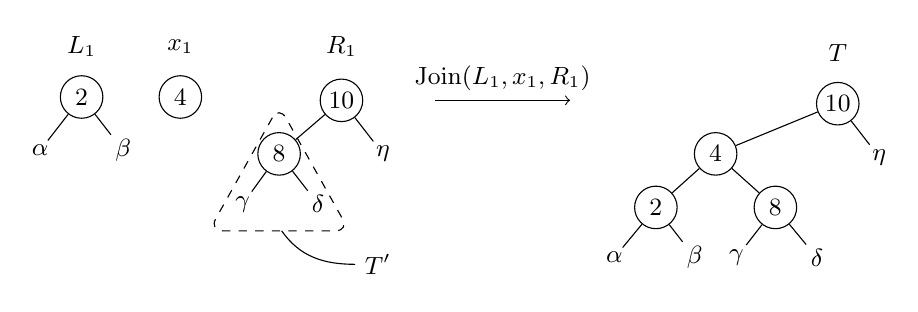
\begin{tikzpicture}[x=0.66cm,y=0.85cm,font=\small,
  n/.style={circle,draw,inner sep=0pt,minimum size=5.4mm},
  g/.style={inner sep=1.5pt}]
  % L1
  \node at (2.5,-0.8) {$L_1$};
  \node[n] (l2) at (2.5,-1.55) {2};
  \node[g] (la) at (1.7,-2.35) {$\alpha$}; \node[g] (lb) at (3.3,-2.35) {$\beta$};
  \draw (l2)--(la) (l2)--(lb);
  % x1
  \node at (4.4,-0.8) {$x_1$};
  \node[n] at (4.4,-1.55) {4};
  % R1
  \node at (7.5,-0.8) {$R_1$};
  \node[n] (r10) at (7.5,-1.6) {10};
  \node[n] (r8) at (6.3,-2.4) {8};
  \node[g] (re) at (8.3,-2.4) {$\eta$};
  \node[g] (rg) at (5.6,-3.15) {$\gamma$}; \node[g] (rd) at (7.05,-3.15) {$\delta$};
  \draw (r10)--(r8) (r10)--(re) (r8)--(rg) (r8)--(rd);
  \draw[dashed,rounded corners=5pt] (6.3,-1.68)--(4.95,-3.55)--(7.65,-3.55)--cycle;
  \node (tp) at (8.2,-4.05) {$T'$};
  \draw (tp.west) to[out=180,in=-55] (6.35,-3.55);
  % Join 箭頭
  \draw[->] (9.3,-1.6)--node[above]{Join($L_1,x_1,R_1$)}(11.9,-1.6);
  % T
  \node at (17.05,-0.9) {$T$};
  \node[n] (t10) at (17.05,-1.65) {10};
  \node[n] (t4) at (14.7,-2.4) {4};
  \node[g] (te) at (17.85,-2.45) {$\eta$};
  \node[n] (t2) at (13.55,-3.2) {2}; \node[n] (t8) at (15.85,-3.2) {8};
  \node[g] (ta) at (12.75,-3.95) {$\alpha$}; \node[g] (tb) at (14.3,-3.95) {$\beta$};
  \node[g] (tg) at (15.1,-3.95) {$\gamma$}; \node[g] (td) at (16.65,-3.95) {$\delta$};
  \draw (t10)--(t4) (t10)--(te) (t4)--(t2) (t4)--(t8) (t2)--(ta) (t2)--(tb) (t8)--(tg) (t8)--(td);
\end{tikzpicture}
\end{center}
Please note that almost all steps, except for (1), have been finalized --- there could be multiple
ways to choose $T'$ in (1). The tree returned from Join($L,x,R$) may not be unique. Additionally,
unlike AVL or Red-Black trees, Join($L,x,R$) does not perform re-coloring and re-balancing. Consider
the following arguments passed into Join($L_2,x_2,R_2$). All nil nodes (considered as leaves in
red-black trees) are omitted for brevity.
\begin{center}
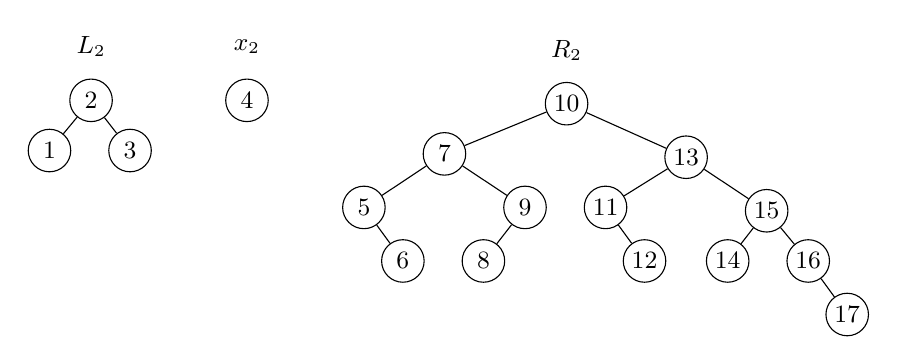
\begin{tikzpicture}[x=0.66cm,y=0.85cm,font=\small,
  n/.style={circle,draw,inner sep=0pt,minimum size=5.4mm}]
  \node at (2.85,-0.75) {$L_2$};
  \node[n] (a2) at (2.85,-1.55) {2};
  \node[n] (a1) at (2.05,-2.3) {1}; \node[n] (a3) at (3.6,-2.3) {3};
  \draw (a2)--(a1) (a2)--(a3);
  \node at (5.85,-0.75) {$x_2$};
  \node[n] at (5.85,-1.55) {4};
  \node at (12,-0.8) {$R_2$};
  \node[n] (r10) at (12,-1.6) {10};
  \node[n] (r7) at (9.65,-2.35) {7};   \node[n] (r13) at (14.3,-2.4) {13};
  \node[n] (r5) at (8.1,-3.15) {5};    \node[n] (r9) at (11.2,-3.15) {9};
  \node[n] (r11) at (12.75,-3.15) {11}; \node[n] (r15) at (15.85,-3.2) {15};
  \node[n] (r6) at (8.85,-3.95) {6};   \node[n] (r8) at (10.4,-3.95) {8};
  \node[n] (r12) at (13.5,-3.95) {12}; \node[n] (r14) at (15.1,-3.95) {14};
  \node[n] (r16) at (16.65,-3.95) {16}; \node[n] (r17) at (17.4,-4.75) {17};
  \draw (r10)--(r7) (r10)--(r13) (r7)--(r5) (r7)--(r9) (r13)--(r11) (r13)--(r15)
        (r5)--(r6) (r9)--(r8) (r11)--(r12) (r15)--(r14) (r15)--(r16) (r16)--(r17);
\end{tikzpicture}
\end{center}
Please select the correct description(s) below.
\begin{enumerate}[label=\Alph*.]
\item If no additional balance is required for $L_2$ and $R_2$, i.e., both $L_2$ and $R_2$ are BSTs,
there are 6 possible tree shapes that could be returned from Join($L_2,x_2,R_2$).
\item If both $L_2$ and $R_2$ are AVL trees as observed, among all possible tree shapes returning
from Join($L_2,x_2,R_2$), there is a unique tree that is an AVL tree.
\item There are multiple ways to assign colors to the nodes in $R_2$ to make $R_2$ a red-black tree.
\item There exists a color assignment to all nodes in $L_2\cup\{x_2\}\cup R_2$ such that: (1) both
$L_2$ and $R_2$ are red-black trees, (2) a red-black tree can be returned from Join($L_2,x_2,R_2$),
and (3) the node with the key 4 is BLACK.
\item There exists a unique color assignment to all nodes in $L_2\cup\{x_2\}\cup R_2$ such that: (1)
both $L_2$ and $R_2$ are red-black trees, (2) a red-black tree can be returned from
Join($L_2,x_2,R_2$), and (3) the node with the key 1 is BLACK.
\end{enumerate}
\end{pastexam}

\begin{pastsoln}
答案：A、E。

\textbf{$T'$ 能選哪些。} 「子樹」指某個節點連同它所有的子孫，或是某個 nil 的位置（空子樹）。
先看 $T'$ 取自 $R$ 的情形。 $T'$ 的鍵都比 $x$ 大，$L$ 的鍵都比 $x$ 小，所以 $x$ 的左子樹是 $L$、
右子樹是 $T'$，再把 $x$ 放回 $T'$ 原來的位置。 若 $T'$ 的某個祖先 $a$ 把 $T'$ 放在\textbf{右}子樹
裡，$x$ 接回去之後也在 $a$ 的右子樹，要 $x.\mathit{key} > a.\mathit{key}$，但 $x$ 比 $R$ 的每個鍵
都小，不行。 所以從 $R$ 的根走到 $T'$ 只能一路往左：$T'$ 是 $R$ 最左那條路徑上某個節點的子樹，
或是最小值左邊的空位置。 反過來，這些位置都可以：$x$ 和 $L$ 的鍵比 $T'$ 所有祖先都小，放在它們的
左子樹裡沒有問題。 對稱地，$T'$ 取自 $L$ 時，只能在 $L$ 最右那條路徑上，$x$ 的左子樹是 $T'$、右子
樹是 $R$。 例題的 $T'$（以 $8$ 為根）就是 $R_1$ 的根的左子樹。

本題 $R_2$ 最左的路徑是 $10 \to 7 \to 5 \to$（$5$ 的左邊是空的），$L_2$ 最右的路徑是
$2 \to 3 \to$（$3$ 的右邊是空的）。 可選的 $T'$ 共 $4 + 3 = 7$ 種：
\begin{center}
\begin{tabular}{clll}
\toprule
 & $T'$ & $x$ 放在哪裡 & $x$ 的左、右子樹 \\
\midrule
(1) & 整棵 $R_2$ 或整棵 $L_2$ & 根 & $L_2$、$R_2$ \\
(2) & 以 $7$ 為根 & $10$ 的左子節點 & $L_2$、以 $7$ 為根 \\
(3) & 以 $5$ 為根 & $7$ 的左子節點 & $L_2$、以 $5$ 為根 \\
(4) & $5$ 左邊的空位置 & $5$ 的左子節點 & $L_2$、空 \\
(5) & 以 $3$ 為根 & $2$ 的右子節點 & 以 $3$ 為根、$R_2$ \\
(6) & $3$ 右邊的空位置 & $3$ 的右子節點 & 空、$R_2$ \\
\bottomrule
\end{tabular}
\end{center}
$T'$ 取整棵 $R_2$ 和取整棵 $L_2$ 得到同一棵樹（$x$ 當根，左 $L_2$ 右 $R_2$），其餘情形 $x$ 的位置都
不同，形狀也不同。

\textbf{A 對。} 由上表，可能的形狀恰好 $6$ 種。

\textbf{B 錯。} 高度以節點數計（空樹 $0$）。 $L_2$ 高 $2$；$R_2$ 裡以 $5$、$7$、$13$ 為根的子樹高
$2$、$3$、$4$，$R_2$ 高 $5$，各節點左右高度差都不超過 $1$，所以 $L_2$、$R_2$ 確實是 AVL 樹。 逐一
檢查六種形狀（沒動到的節點，子樹不變，平衡不變；只需看 $x$ 和它的祖先）：
\begin{itemize}
\item (1) $x$ 的左右高度 $2$、$5$，差 $3$。 不是。
\item (2) $x$ 的左右高度 $2$、$3$，$x$ 高 $4$；$10$ 的左右高度 $4$、$4$。 是 AVL 樹。
\item (3) $x$ 的左右高度 $2$、$2$，$x$ 高 $3$；$7$ 的左右高度 $3$、$2$（以 $9$ 為根），高 $4$；$10$ 的
左右 $4$、$4$。 也是 AVL 樹。
\item (4) $x$ 的左右高度 $2$、$0$。 不是。
\item (5)(6) $x$ 的左右高度 $1$、$5$ 或 $0$、$5$。 不是。
\end{itemize}
有兩棵是 AVL 樹，不是唯一。

\textbf{C 錯。} 紅黑樹的性質（資結書定義~10.2）：根是黑的、紅節點的子節點是黑的、從任一節點到它
底下每個 nil 的路徑上黑節點數相同。 以下「黑數」指從根到某個 nil 的路徑上的黑節點數（不算 nil），
$R_2$ 的每條路徑黑數都要相同，記為 $B$。
\begin{itemize}
\item 路徑 $10, 7, 5$（到 $5$ 左邊的 nil）只有 $3$ 個節點，所以 $B \le 3$。
\item 路徑 $10, 13, 15, 16, 17$ 有 $5$ 個節點，根是黑的；$13, 15, 16, 17$ 這四個裡紅的不能相鄰，最多
$2$ 個紅，所以黑數至少 $3$，$B \ge 3$。
\item 於是 $B = 3$：$10, 7, 5$ 都是黑的，而且 $13, 15, 16, 17$ 恰好兩紅兩黑。
\item 路徑 $10, 13, 11$（到 $11$ 左邊的 nil）只有 $3$ 個節點，全黑：$13$、$11$ 黑。 那麼
$15, 16, 17$ 裡要兩紅且不相鄰，只能 $15$、$17$ 紅，$16$ 黑。
\item 其餘的也被定下來：路徑 $10, 7, 9$ 只有 $3$ 個節點，$9$ 黑；$10, 7, 9, 8$ 已有 $3$ 黑，$8$ 紅；
同理 $6$ 紅（$10, 7, 5$ 已 $3$ 黑）、$12$ 紅（$10, 13, 11$ 已 $3$ 黑）；$10, 13, 15, 14$ 中 $15$ 紅，
要 $3$ 黑，$14$ 黑。
\end{itemize}
檢查一下紅節點 $6, 8, 12, 15, 17$ 的子節點都是黑的（或 nil），成立。 所以 $R_2$ 的著色是唯一的：
黑 $= \{10, 7, 5, 9, 13, 11, 16, 14\}$，紅 $= \{6, 8, 12, 15, 17\}$。 （如果採用允許根是紅色的定義，
會多出一種著色；本書照資結書的定義，根一定是黑的。）

\textbf{D 錯。} $L_2$ 的著色：$2$ 黑，$1$、$3$ 同色（兩邊黑數要一樣）。 兩個都紅時 $L_2$ 的黑數是
$1$，兩個都黑時是 $2$。 Join 不重新著色，$x$ 放進 $T'$ 原來的位置後，以 $x$ 為根的子樹的黑數必須等於
$T'$ 原來的黑數，$x$ 的兩棵子樹黑數也要相等。 $R_2$ 裡：整棵 $3$、以 $7$ 為根 $2$、以 $5$ 為根 $1$、
空位置 $0$。
\begin{itemize}
\item (1) $x$ 的兩棵子樹是 $L_2$（黑數 $\le 2$）和 $R_2$（黑數 $3$），不相等。 不行。
\item (2) $x$ 的子樹是 $L_2$ 和以 $7$ 為根（黑數 $2$），所以 $1$、$3$ 黑；以 $x$ 為根的黑數要等於原來的
$2$，$x$ 必須是紅的。 $x$ 的父節點 $10$、子節點 $2$、$7$ 都黑，可以。
\item (3) $x$ 的子樹是 $L_2$ 和以 $5$ 為根（黑數 $1$），所以 $1$、$3$ 紅；以 $x$ 為根的黑數要等於 $1$，
$x$ 必須是紅的。 父節點 $7$、子節點 $2$、$5$ 都黑，可以。
\item (4) 以 $x$ 為根的黑數至少是 $L_2$ 的黑數 $\ge 1$，原來的位置黑數 $0$。 不行。
\item (5)(6) $x$ 在 $L_2$ 裡面，$x$ 的子樹包含整棵 $R_2$，從根 $2$ 經過 $x$ 再走進 $R_2$ 的路徑黑數至少
$1 + 3 = 4$，但路徑 $2, 1$ 的黑數最多 $2$。 不行。
\end{itemize}
能得到紅黑樹的只有 (2)、(3)，兩者的 $4$ 都是紅的，所以不存在讓 $4$ 是黑色的著色。

\textbf{E 對。} 要 $1$ 是黑的，$L_2$ 只能是 $2$、$1$、$3$ 全黑，由上面的分析只剩 (2)，而且 $x$ 必須是
紅的；$R_2$ 的著色由 C 已經唯一確定。 所以滿足條件的著色恰好一種，Join 回傳的就是下面這棵（黑節點
塗黑，紅節點塗紅）：
\begin{center}
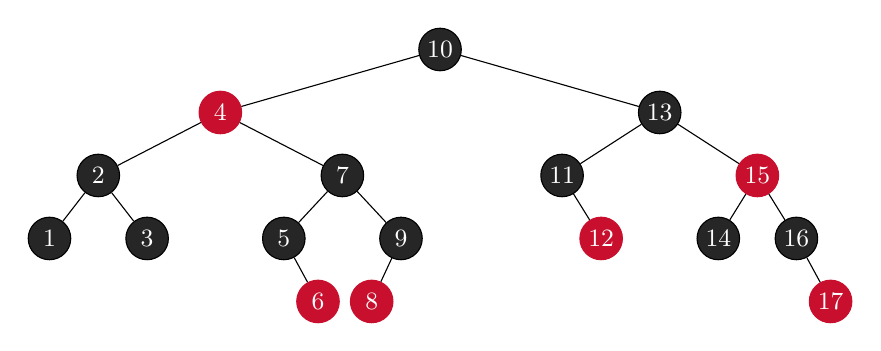
\begin{tikzpicture}[x=0.62cm,y=0.8cm,font=\small,
  b/.style={circle,draw=black,fill=black!85,text=white,inner sep=0pt,minimum size=5.4mm},
  r/.style={circle,draw={rgb,255:red,200;green,16;blue,46},fill={rgb,255:red,200;green,16;blue,46},
            text=white,inner sep=0pt,minimum size=5.4mm}]
  \node[b] (n10) at (9,0) {10};
  \node[r] (n4) at (4.5,-1) {4};      \node[b] (n13) at (13.5,-1) {13};
  \node[b] (n2) at (2,-2) {2};        \node[b] (n7) at (7,-2) {7};
  \node[b] (n11) at (11.5,-2) {11};   \node[r] (n15) at (15.5,-2) {15};
  \node[b] (n1) at (1,-3) {1};        \node[b] (n3) at (3,-3) {3};
  \node[b] (n5) at (5.8,-3) {5};      \node[b] (n9) at (8.2,-3) {9};
  \node[r] (n12) at (12.3,-3) {12};   \node[b] (n14) at (14.7,-3) {14};
  \node[b] (n16) at (16.3,-3) {16};
  \node[r] (n6) at (6.5,-4) {6};      \node[r] (n8) at (7.6,-4) {8};
  \node[r] (n17) at (17,-4) {17};
  \draw (n10)--(n4) (n10)--(n13) (n4)--(n2) (n4)--(n7) (n2)--(n1) (n2)--(n3)
        (n7)--(n5) (n7)--(n9) (n5)--(n6) (n9)--(n8) (n13)--(n11) (n13)--(n15)
        (n11)--(n12) (n15)--(n14) (n15)--(n16) (n16)--(n17);
\end{tikzpicture}
\end{center}
每條從根到 nil 的路徑恰有 $3$ 個黑節點，紅節點 $4, 6, 8, 12, 15, 17$ 的子節點都是黑的。
\end{pastsoln}
